\documentclass{article}
\usepackage[utf8]{inputenc}
\usepackage[spanish]{babel}
\usepackage{listings}
\usepackage{graphicx}
\graphicspath{ {images/} }
\usepackage{cite}

\begin{document}

\begin{titlepage}
    \begin{center}
        \vspace*{1cm}
            
        \Huge
        \textbf{Ideación Proyecto Final -Segunda Entrega }

        \vspace{0.5cm}
        \LARGE
        I'm Alive
            
        \vspace{1.5cm}
            
        \textbf{Sergio Alberto Giraldo Salazar y Esteban Felipe Güiza Piñeros}
            
        \vfill
            
        \vspace{0.8cm}
            
        \Large
        Despartamento de Ingeniería Electrónica y Telecomunicaciones\\
        Universidad de Antioquia\\
        Medellín\\
        Septiembre de 2021
            
    \end{center}
\end{titlepage}

\tableofcontents
\newpage
\section{Idea del Juego}\label{idea}
El juego va a tratar de un androide el cual desarrollo conciencia propia y desea vivir una vida como un ser autónomo e independiente, para lograr su sueño debe escapar del laboratorio donde fue creado, ya que fue creado para ser un arma de destrucción.
\cite{Alaluzdeunabombilla}

\section{Personajes Principales} \label{personajes}
\begin{itemize}
    \item Androide (personaje principal).
    \item Segundo Androide (sólo si es multijugador).
\end{itemize}

\section{Enemigos}\label{enemigos}
\begin{itemize}
    \item Soldados: Estos enemigos atacaran al personaje quitándole vidas, algunos soltaran ítems como vidas.
    \item Científicos: Estos atacarán al androide y de ser derrotados podrán soltar llaves para avanzar a la siguiente habitación. 
\end{itemize}

\section{Mapa}\label{mapa}
El juego va a contar con un mapa de un laboratorio subterráneo, el cual estará dividido en 5 niveles que serían los 5 pisos del laboratorio, y para poder avanzar de nivel deberás derrotar todos los enemigos de una habitación para recibir la llave y poder pasar a la siguiente, cuando halles la habitación indicada encontraras el ascensor para avanzar a un nuevo piso. 

\begin{figure}[h]
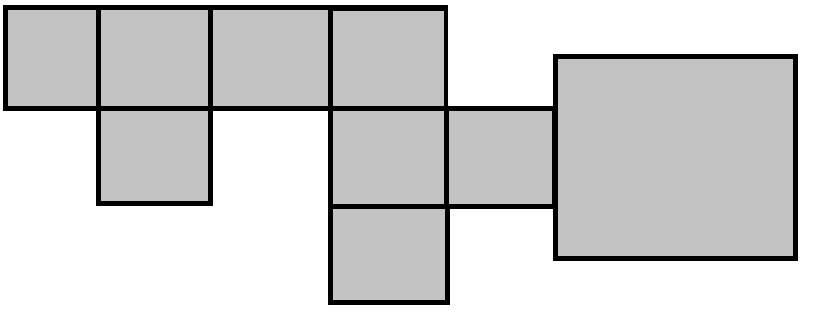
\includegraphics[width=8cm]{01.png}
\centering
\caption{Mapa del juego}
\label{fig:cpplogo}
\end{figure}

\begin{itemize}
    \item  sería un bosquejo del mapa de capa piso, cada cuadro representa una habitación del laboratorio, en total serian 5 mapas con este diseño (uno para cada piso)
\end{itemize}
\newpage


\section{Modo de Juego}\label{modo}
\begin{itemize}
    \item \textbf{Perspectiva:} Top-Down.
    \item \textbf{Modo de combate:}Disparar proyectiles los cuales se detienen hasta que impacten un soldado o un muro, esquivar los proyectiles de los soldados ya que estos te quitaran una vida. Deberás derrotar todos los enemigos de una habitación para obtener las tarjetas para abrir las puertas.
    \item \textbf{Información en pantalla:}Te podrás desplazar en 8 direcciones, en la pantalla hallaras en la parte de abajo a la izquierda la cantidad de vidas que te quedan, en la parte superior en medio encontrar la información de la partida y en la parte inferior derecha un mapa del piso en el que estas. En las habitaciones habrán objetos decorativos que podrás usar para cubrirte de los enemigos y puertas en algunos de los muros. 

\begin{figure}[h]
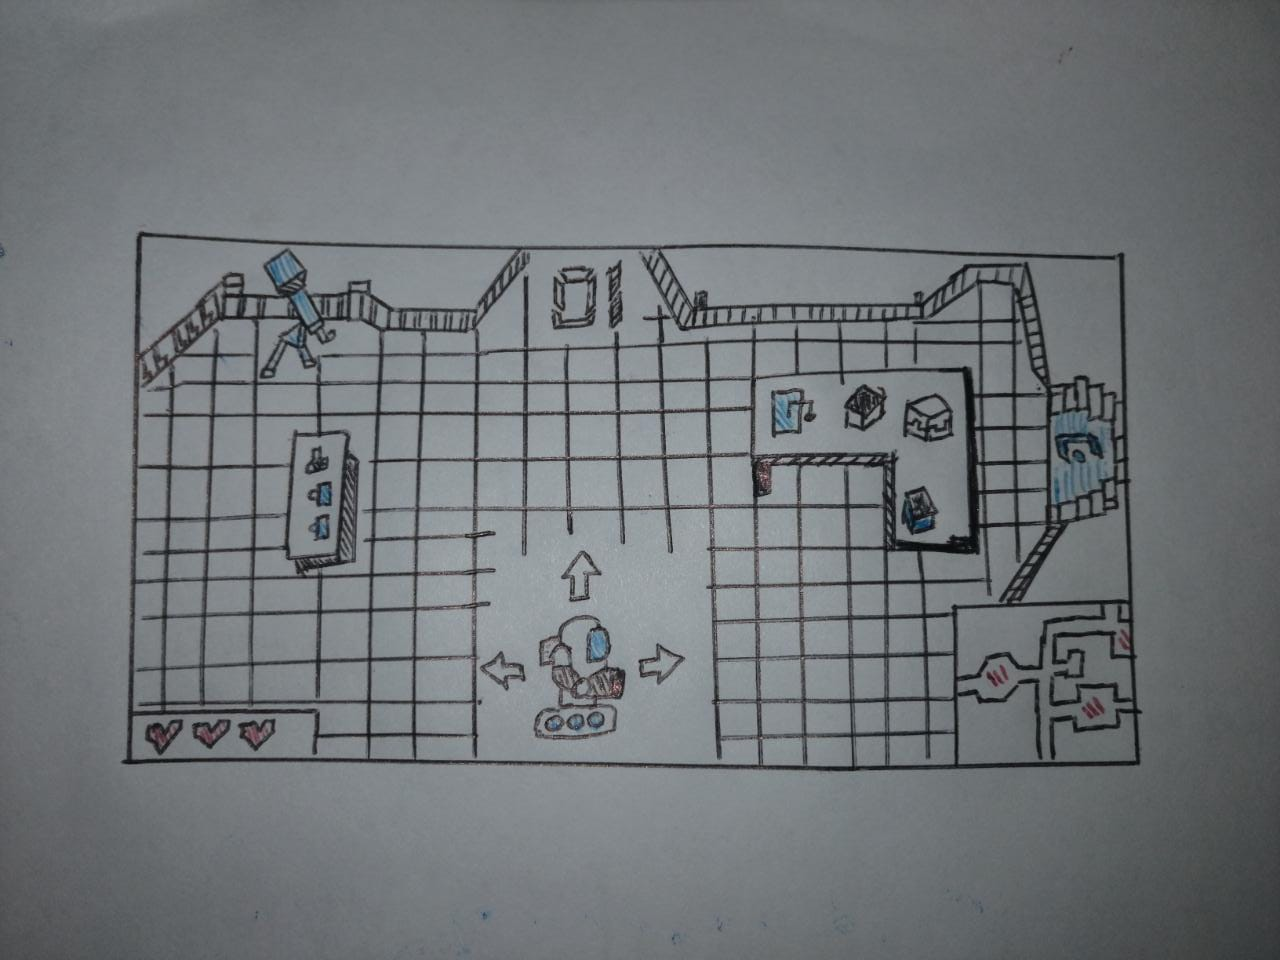
\includegraphics[width=8cm]{02.jpg}
\centering
\caption{Diseño de pantalla}
\label{fig:cpplogo}
\end{figure}

\end{itemize}

\section{Nivel de Dificultad}\label{dificultad}
La dificultad ira aumentando junto con los niveles. Esto se hará incrementando la cantidad de enemigos, cadencia de fuego y puntos de vida de los enemigos.

\section{Gráficos}\label{gráficos}
se haran diseños 2D 
\section{Tipo de perspectiva}\label{gráficos}
se visualiza en una perspectiva top Down y el jugador se podrá mover en 8 direcciones

\bibliographystyle{IEEEtran}
\bibliography{references}

\end{document}
